\input{~/macro.tex}
\title{定常的とみなせる外力が加わった際の荷電粒子の運動}
\author{20B01392 松本侑真}
\date{\today}
\begin{document}
\maketitle
\begin{abstract}
	プラズマ物理学において、定常的な外力が加わった差異の荷電粒子の運動についてまとめる。
	また、外力が時間的に変化している場合においても、粒子のサイクロトロン運動よりも十分にゆっくりであれば成立する。
\end{abstract}
\tableofcontents
\newpage

\section{一様定常磁場と定常的な外力}
荷電粒子に対して一様定常磁場$\bm{B}$と定常的な外力$\bm{F}(\bm{x})$が印加している場合を考える。
まずは、粒子の速度ベクトルを磁場$\bm{B}$に垂直な方向と平行な方向へと分解する:
\begin{equation}
	\bm{v} = \bm{v}_{\perp} + \bm{v}_{\parallel}\;。
\end{equation}
外力の磁場に平行な成分については、大きさが$\bm{F}_{\parallel}/m$の等加速度直線運動を与えるだけである。
そのため、以下では磁場$\bm{B}$と垂直な成分のみを考える($\bm{F} = \bm{F}_{\perp}$)。このとき、磁場に垂直な方向における荷電粒子の運動方程式は
\begin{equation}
	m\dot{\bm{v}}_{\perp} = q\qty(\bm{v}_{\perp}\cross\bm{B}) + \bm{F}_{\perp}
	\label{eq:mv_all}
\end{equation}
となる。外力が加わっていない場合、磁場$\bm{B}$に垂直な方向において荷電粒子は円運動を行うことが直ちにわかる。そのため、$\bm{v}_{\perp}$を$\bm{v}_0$(円運動成分)と$\bm{v}_{\text{F}}$(ドリフト運動成分)に分解して考える。
\footnote{ローレンツ力と外力が張る平面が磁場と垂直であるため、$\bm{v}_{\parallel}$方向に$\bm{v}_{\text{F}}$は存在しない。}
このとき、円運動成分については以下の運動方程式が成立している:
\begin{equation}
	m\dot{\bm{v}}_0 = q\qty(\bm{v}_0\cross\bm{B})\;。
\end{equation}
定常的な外力が印加されていることから、$\bm{v}_{\text{F}}$の時間変化がないと考えて良い\footnote{円運動について平均を取ると直流成分のみが残り、それが$\bm{v}_{\text{F}}$となるはずだから、時間変化はないと考えて良い。}ため、
式\eqref{eq:mv_all}は
\begin{equation}
	m\dot{\bm{v}}_0 = q\qty(\bm{v}_0\cross\bm{B}) + q\qty(\bm{v}_{\text{F}}\cross\bm{B}) + \bm{F}_{\perp}
\end{equation}
と書き直すことができる。したがって、
\begin{equation}
	q\qty(\bm{v}_{\text{F}}\cross\bm{B}) + \bm{F}_{\perp} = \bm{0}
\end{equation}
が成立している。右から$\bm{B}$の外積を取ってみると、$(\bm{a}\cross \bm{b})\cross \bm{c} = (\bm{a}\cdot \bm{c})\bm{b} - (\bm{b}\cdot \bm{c})\bm{a}$を用いて、
\begin{equation}
	q\qty(\bm{v}_{\text{F}}\cross\bm{B})\cross\bm{B} = -qB^2\bm{v}_{\text{F}} = -\bm{F}_{\perp}\cross\bm{B}
\end{equation}
となる。したがって、ドリフト運動$\bm{v}_{\text{F}}$は
\begin{equation}
	\bm{v}_{\text{F}} = \frac{\bm{F}_{\perp}\cross\bm{B}}{qB^2} = \frac{\bm{F}\cross\bm{B}}{qB^2}
	\label{eq:drift}
\end{equation}
と求まる。つまり、定常的な外力が加わっている方向には運動しない。
\subsection{定常的な電場が印加されているとき}
例として定常的な電場$\bm{E}$が印加されている場合には、ドリフト運動は電荷に依らないことがわかる。
式\eqref{eq:drift}によると、
\begin{equation}
	\bm{v}_{\bm{E}} = \frac{\bm{E}\cross\bm{B}}{B^2}
\end{equation}
となるため、プラズマ中の電子とイオンは同じ速度で同じ方向にドリフトする。そのため、プラズマ中に電離が生じることがなく、電流は流れない。
また、プラズマ全体は磁力線を横切ってドリフトしていくことがわかる。

\newpage
\section{空間的に変化する定常磁場}
\subsection{磁場と垂直な方向に勾配が生じている場合}
次に、磁場が空間的に変化する場合を考えよう。磁場$\bm{B}$は$z$成分のみを持つするとして、その強さが$y$依存性を持つとする:
\begin{equation}
	\bm{B} =
	\begin{pmatrix}
		0 & 0 & B(y)
	\end{pmatrix}^\top\;。
\end{equation}
\begin{figure}[H]
	\centering
	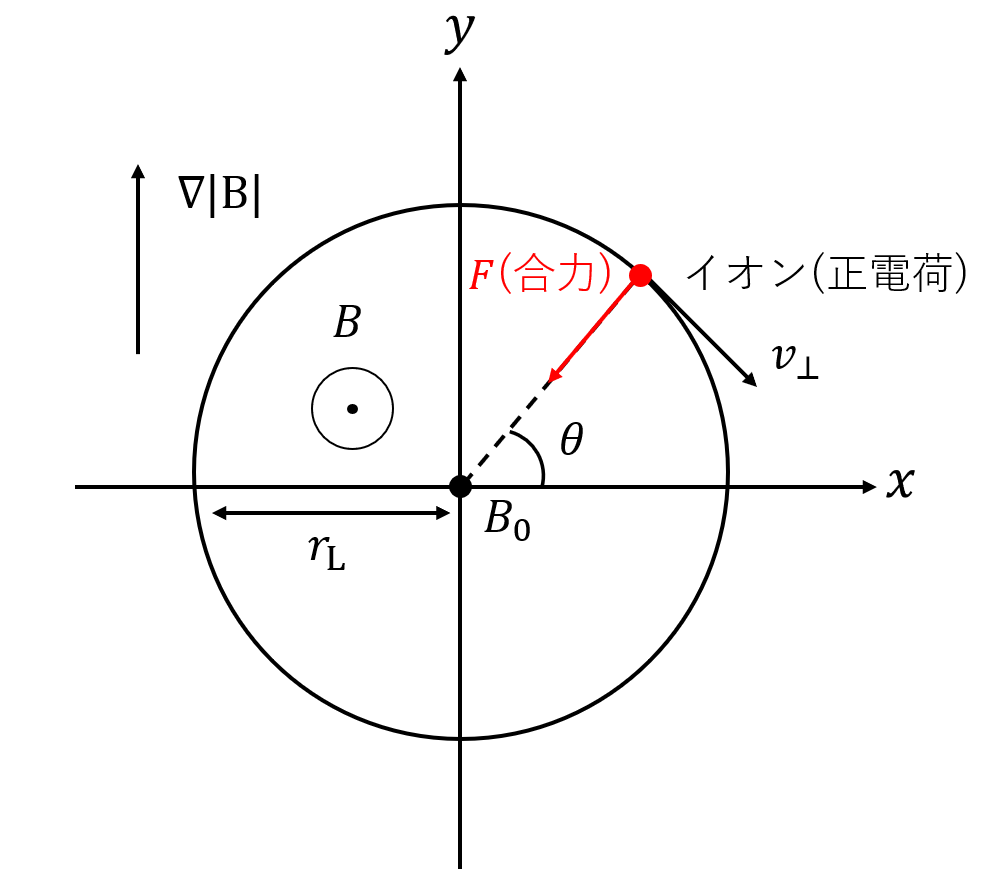
\includegraphics[width=0.6\linewidth]{gradB.png}
	\caption{磁場と垂直な方向に勾配が生じている場合}
	\label{fig:gradB}
\end{figure}
また、$B(y)$は緩やかに変化しているとする。すなわち、回転中心におけるTaylor展開の1次項までで近似できるとする:
\begin{equation}
	B(y) = B_0 + \qty(\pdv{B}{y})_0y = B_0 + \qty(\pdv{B}{y})_0r_{\text{L}}\sin\theta\;。
\end{equation}
ここで、$r_{\text{L}}$はLarmor半径であり、大きさ$B$の定常磁場のみが印加されている際の粒子の磁場に直交する速度成分の大きさを$v_{\perp}$として、$r_{\text{L}} = mv_{\perp}/qB$と表される。
また、回転中心における磁場の大きさを$B_0$とした。さらに、粒子が1旋回する間では磁場の変化が微小であると仮定しているため、$y = r_{\text{L}}\sin\theta$が成立している。
粒子にかかる力について、1旋回に関する平均値を取るとLarmor円運動に関する成分は$0$になるため、磁場の変化によって生じる成分が残る。これを定常的な外力$\bm{F}$とみなすこととする。
1旋回中のイオンにかかるLorentz力を考える。$v_x = v_{\perp}\cos\theta,\,v_y = -v_{\perp}\sin\theta$であることに注意すると、$F_x,\,F_y$は以下のように計算できる:
\begin{align}
	F_x & = qv_yB_z = -qv_{\perp}\cos\theta B(y) = -qv_{\perp}\cos\theta\qty(B_0 + \qty(\pdv{B}{y})_0r_{\text{L}}\sin\theta)\;,  \\
	F_y & = -qv_xB_z = -qv_{\perp}\sin\theta B(y) = -qv_{\perp}\sin\theta\qty(B_0 + \qty(\pdv{B}{y})_0r_{\text{L}}\sin\theta)\;。
\end{align}
したがって、$\bar{F}_x = 0,\,\bar{F}_y \neq 0$となることがわかる。実際に計算すると、
\begin{equation}
	\bar{F}_y = -qv_{\perp}r_{\text{L}}\qty(\pdv{B}{y})_0\frac{1}{2\pi}\int_0^{2\pi}\sin^2\theta\dd{\theta}
	= -\frac{1}{2}qv_{\perp}r_{\text{L}}\qty(\pdv{B}{y})_0 = -\frac{mv^2_{\perp}/2}{B_0}\qty(\pdv{B}{y})_0
\end{equation}
となるため、磁気モーメント$\mu_m \coloneqq mv^2_{\perp}/(2B)$を用いて、一定の外力$F_y = -\mu_m\qty(\pdv*{B}{y})$がイオンの運動中に印加されていると考えて良いことがわかる。
磁場に垂直な一般の方向に対する変化に拡張するのは容易であり、
\begin{equation}
	\bm{F} = -\mu_m\qty(\grad{B})_{\perp}
\end{equation}
と表される。なお、磁気モーメントとは、電流が旋回しているときの面積と電流の積であるため、
\begin{equation}
	\mu_m = SI = \pi r_{\text{L}}^2\times q\qty(\frac{\omega_c}{2\pi}) = \qty(r_{\text{L}}\omega_c)^2\frac{m}{qB}\frac{q}{2} = \frac{mv_{\perp}^2/2}{B}
\end{equation}
のようにして求められる値である。
話を戻して、磁場の垂直方向の勾配によって生じる外力のドリフト速度は
\begin{equation}
	\bm{v}_{B} = \frac{-\mu_m\qty(\grad{B})_{\perp}\cross\bm{B}}{qB^2} = \frac{\mu_m\bm{B}\cross\grad{B}}{qB^2}
\end{equation}
となる。これをgradBドリフトと呼ぶ。
\subsection{湾曲磁場について}

\subsection{磁場と平行な方向に勾配が生じている場合}

\section{一様定常磁場と時間的に緩やかに変化する一様電場}
\section{一様定常磁場と時間的に定常で緩やかに空間変化する電場}


\end{document}